%%%%%%%%%%%%%%%%%%%%%%%%%%%%%%%%%%%%%%%%%%%%%%%%%%%%%%%%%%%%%%%
%
% Welcome to Overleaf --- just edit your LaTeX on the left,
% and we'll compile it for you on the right. If you open the
% 'Share' menu, you can invite other users to edit at the same
\documentclass[10pt]{standalone}
\usepackage{tikz} 
\usetikzlibrary{shapes.geometric}
\begin{document}
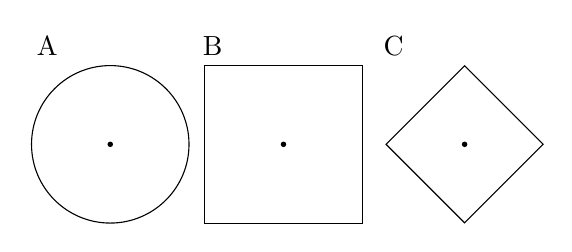
\begin{tikzpicture} 
%\draw[step=1,help lines] ( -5-5 ) grid ( 5, 5); 
\node[above] at (-0.8,1){A};
\draw (0,0) circle (1); %画圆
\fill (0,0) circle (1pt);%画点
%\draw (0,0) ellipse (2 and 1 );%画椭圆 
\node[above] at (1.3,1){B};
\draw[color=black] (1.2,-1) rectangle (3.2,1);%画长方形
\fill (2.2,0) circle (1pt);
\node[diamond,draw,minimum width=2cm,minimum height=2cm] (d) at (4.5,0) {};
\node[above] at (3.6,1){C};
\fill (4.5,0) circle (1pt);
\end{tikzpicture}
\end{document}